\documentclass[12pt,a4paper]{article}

\usepackage[utf8]{inputenc}
\usepackage[T2A]{fontenc}
\usepackage[ukrainian]{babel}
\usepackage{geometry}
\geometry{
    left=2cm,
    right=2cm,
    top=2cm,
    bottom=2cm
}

\usepackage[table]{xcolor}
\usepackage{amsmath}
\usepackage{graphicx}
\usepackage{subcaption} % обов'язково в преамбулі
\usepackage{multirow}  % Для об'єднання рядків
\usepackage{makecell}         % для багато­рядкових комірок
\usepackage{pdflscape}       % або можна використати lscape

\begin{document}

    \begin{titlepage}

        \thispagestyle{empty}
        \begin{center}
        \large
        Національний технічний університет України\\
        «Київський політехнічний інститут імені Ігоря Сікорського»\\[1em]
        Факультет інформатики та обчислювальної техніки\\
        Кафедра обчислювальної техніки
        \end{center}

        \vfill

        \begin{center}
        \textbf{\LARGE Комп'ютерна логіка. Частина 2}\\[2em]
        \textbf{\Large Лабораторна робота №5}\\
        «Дослідження операцій з числами у форматі з плаваючою комою» 
        \end{center}

        \vfill

        \begin{flushright}
        Виконав: студент 1 курсу ФІОТ, гр. ІО-41\\
        \textit{Давидчук А. М.}\\
        Залікова книжка № 4106\\[1em]
        Перевірив: \textit{Верба О.\,А.}
        \end{flushright}

        \vfill

        \begin{center}
        Київ -- 2025
        \end{center}

    \end{titlepage}

    \setlength{\parindent}{0pt}

    \textbf{\underline{Тема:}} «Дослідження операцій з числами у форматі з плаваючою комою».

    \vspace{1em}
    
    \textbf{\underline{Мета:}} Дослідити машинні методи виконання операцій з числами в форматі з плаваючою комою.

    \begin{center} \textbf{\large Виконання роботи} \end{center}

    \vspace{1em}

    \setlength{\parindent}{1.5em}

    Мій номер залікової книжки: 4106, що у двіковому вигляді є 0001 0000 0000 1010.
    Звідси $x_9 = 0, x_8 = 0, x_7 = 0, x_6 = 0, x_5 = 0, x_4 = 1, x_3 = 0, x_2 = 1, x_1 = 0$.
    Звідси визначу два числа $X$ та $Y$:

    \vspace{1em}

    $X = -x_7x_61x_5x_40,x_31x_2x_1 = -001010,0110$,

    $Y = +x_91x_8x_7,x_6x_5x_4x_3x_2x_1 = +0100,001010$

    Також визначу способи виконання двох операцій множення, однієї операції ділення та додавання:

    \begin{table}[h!]
        \centering
        \begin{tabular}{|c|c|c|c|c|l|}
        \hline
        $x_2, x_1$ & Спосіб множення & $x_3$ & Спосіб ділення & $x_5, x_4$ & Машинні коди в АЛУ \\
        \hline
        00 & 1-й, 4-й & \cellcolor{yellow!30}0 & \cellcolor{yellow!30}1-й & 00 & Додавання в ОК \\
        01 & 2-й, 3-й & 1 & 2-й & \cellcolor{yellow!30}01 & \cellcolor{yellow!30}Додавання в ДК \\
        10 \cellcolor{yellow!30}& \cellcolor{yellow!30}1-й, 3-й & \empty & 1-й & 10 & Віднімання в ОК \\
        11 & 2-й, 4-й & \empty & 2-й & 11 & Віднімання в ДК \\
        \hline
        \end{tabular}
    \end{table}

    Тобто у мене 1-й та 3-й спосіб множення, 1-й спосіб ділення та додавання в ДК.

    Тепер подам числа $X$ та $Y$ у форматі з плаваючою комою, шляхом переміщення «фіксованої» коми перед старшим бітом мантиси, і відповідним значенням порядка (для порядку я виділю 4 біти, що буде достатнім для цієї лабораторної роботи):
    \begin{flalign*}
        &
        \begin{array}{r@{\ =\ }c c c c}
        X & \fbox{0}     & \fbox{0110} & \fbox{1} & \fbox{0010100110} \\
        Y & \fbox{0}     & \fbox{0100} & \fbox{0} & \fbox{0100001010}
        \end{array}
        &
    \end{flalign*}

    Так як мантиса подаєтсья у вигляді [знак; модуль], то значить ми можемо говорити про нормалізацію мантис як додатніх мантис, які у старшому розряді завжди мають 1.
    Але як видно, мантиси чисел $X$ та $Y$ не задовільняють нормалізованого вигляду, тому проведемо нормалізацію мантис шляхом зсуву вліво на $n$ кількість бітів і віднімання порядку на $n$,
    поки не буде досягнуто нормалізованої мантиси:
    \begin{flalign*}
        &
        \begin{array}{r@{\ =\ }c c c c}
        X & \fbox{0}     & \fbox{0100} & \fbox{1} & \fbox{1010011000} \\
        Y & \fbox{0}     & \fbox{0011} & \fbox{0} & \fbox{1000010100}
        \end{array}
        &
    \end{flalign*}

    Тепер подам числа $X$ та $Y$ за стандартом ANSI/IEEE 754-2008 в короткому 32-бітному форматі. Для цього потрібно знайти зміщенний порядок (8 бітів), а також розширити мантису до 23 бітів:

    \vspace{1em}

    $X: P_{\text{зміщ}} = P + (2^{8-1} - 1)_{10} = P + 127_{10} = 4_{10} + 127_{10} = 131_{10} = 10000011_2$, тоді

    $X_{\text{к. ф.}} = 1.10000011,10100110000000000000000$

    \vspace{1em}

    $Y: P_{\text{зміщ}} = P + (2^{8-1} - 1)_{10} = P + 127_{10} = 3_{10} + 127_{10} = 130_{10} = 10000010_2$, тоді

    $Y_{\text{к. ф.}} = 0.10000010,10000101000000000000000$

    \vspace{1em}

    Перейдімо до виконання операцій над числами у форматі з плаваючою комою.

    \newpage

    Але перж ніж перейти вже до виконання операцій, ми маємо узгодити розрядність мантис та операційних пристроях.
    В даній лабораторній роботі на мантису відводиться 7 розрядів (з урахуванням знакового) --- тому я округлю мантису $X$ до 6 розрядів (без урахування знакового):

    \begin{flalign*}
        &
        \begin{array}{r}
        M_X: 1010011 \\
        + \phantom{1\ }0000001 \\
        \hline
        1010100
        \end{array}
        &
    \end{flalign*}

    \setlength{\parindent}{0pt}

    Тобто $M_X \approx 101010$, а $M_Y \approx 100001$. Тоді

    \begin{flalign*}
        &
        \begin{array}{r@{\ =\ }c c c c}
        X & \fbox{0}     & \fbox{0100} & \fbox{1} & \fbox{101010} \\
        Y & \fbox{0}     & \fbox{0011} & \fbox{0} & \fbox{100001}
        \end{array}
        &
    \end{flalign*}

    \textbf{\Large Множення:}

    \vspace{1em}

    \text{\large Теоретичне підґрунтя:}

    \setlength{\parindent}{1.5em}

    \vspace{1em}

    Дано два числа: $X = 2^a M_X$ та $Y = 2^b M_Y$.

    Під час множення двох чисел отримаємо: $X \cdot Y = 2^a M_X \cdot 2^b M_Y = 2^{a + b} \left( M_X \cdot M_Y \right)$.

    Тобто при множенні двох чисел у форматі з плаваючою комою: додаються порядки, множаться мантиси цих чисел.

    \vspace{1em}
    \setlength{\parindent}{0pt}

    \textbf{\large Множення 1-й спосіб:}

    \vspace{1em}

    Операційна схема множення 1-го способу для 6 розрядних чисел:

    \begin{figure}[ht]
        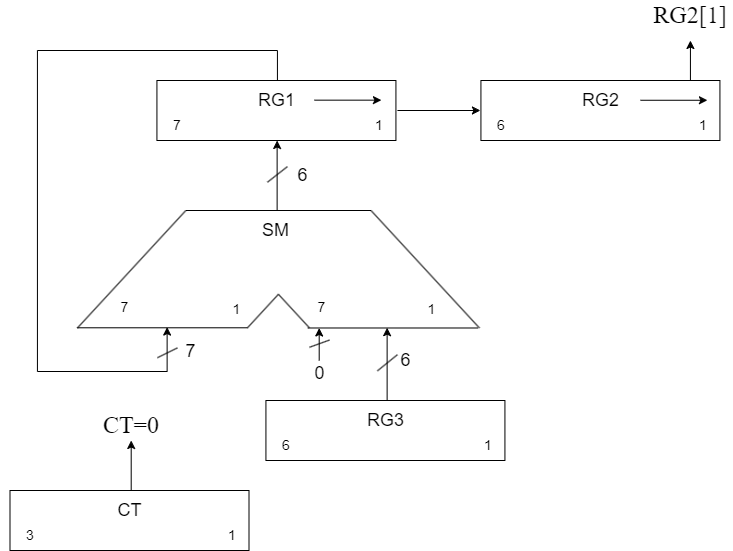
\includegraphics[width=0.8\textwidth]{multiply1_operation_schemma.png}
    \end{figure}

    \newpage

    Змістовний та ФС мікроалгоритми:

    \begin{figure}[h!]
        \centering
        
        \begin{subfigure}[t]{0.45\textwidth}
            \centering
            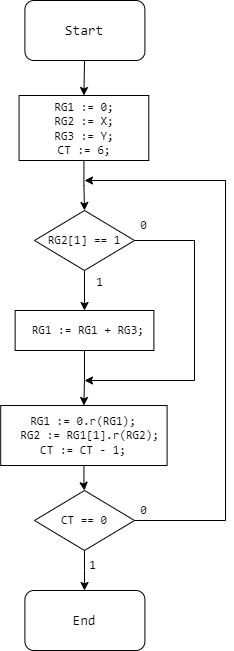
\includegraphics[width=\linewidth]{structure_alg.png}
        \end{subfigure}
        \hfill
        \begin{subfigure}[t]{0.45\textwidth}
            \centering
            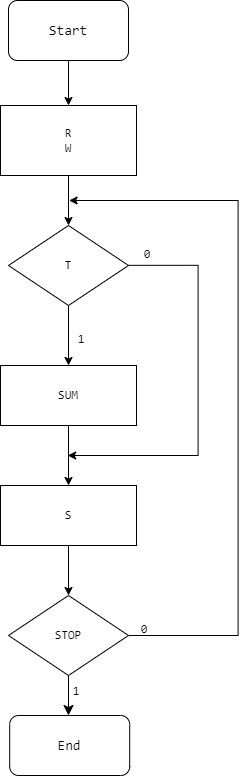
\includegraphics[width=\linewidth]{FS_alg.png}
        \end{subfigure}
        
        \label{fig:microalg}

    \end{figure}

    \newpage

    TABLE 1

    \newpage

    Функціональна схема множення, в якій використовується 8-бітний регістр та суматор для зручності:

    \begin{figure}[ht]
        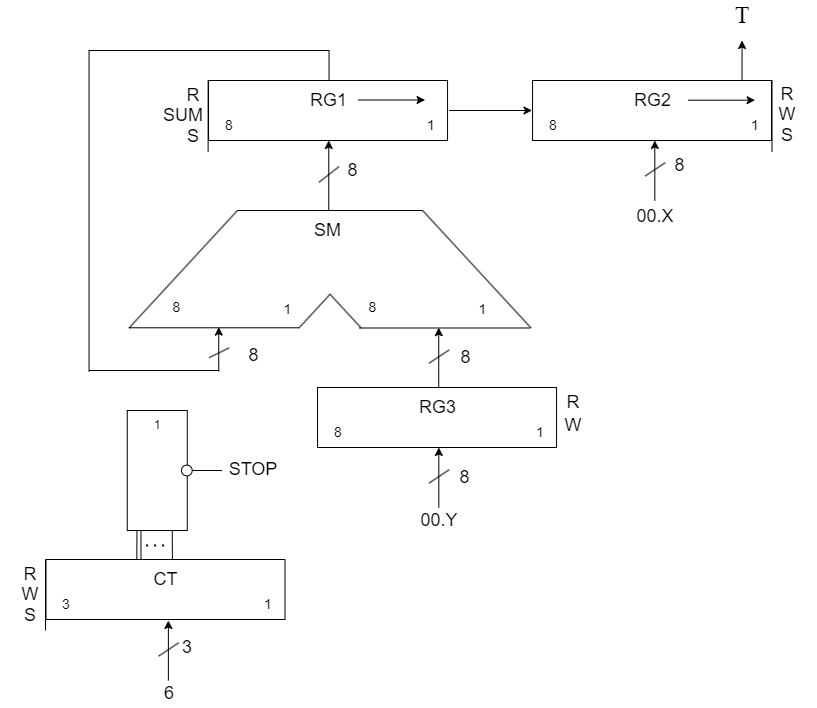
\includegraphics[width=0.8\textwidth]{multiply1_function_schemma.png}
    \end{figure}

    \newpage

    Схема AFDK:

    \begin{figure}[ht]
        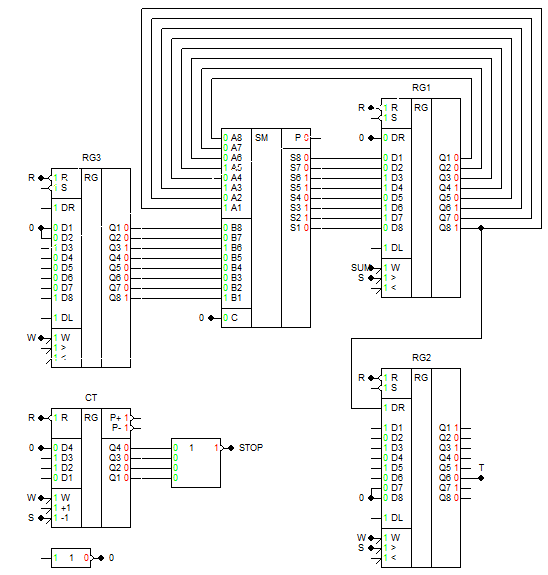
\includegraphics[width=0.7\textwidth]{schemma1.png}
    \end{figure}

    Часова діаграма:

    \begin{figure}[ht]
        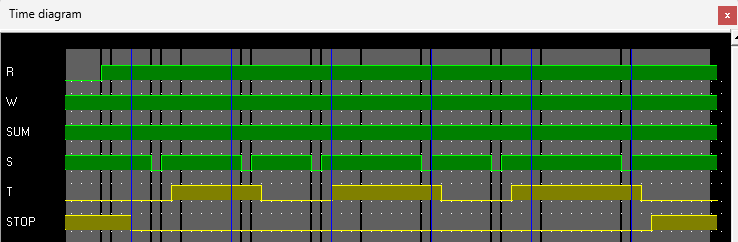
\includegraphics[width=1.0\textwidth]{time1.png}
    \end{figure}

    Результат множення збігається з попередньо обчисленим.

    \newpage

    \textbf{\large Множення 3-й спосіб:}

    \vspace{1em}

    Операційна схема множення 3-го способу для 6 розрядних чисел:

    \begin{figure}[ht]
        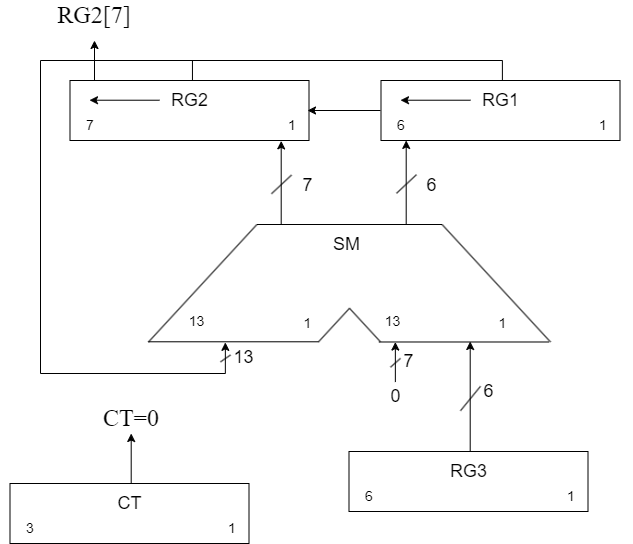
\includegraphics[width=1.0\textwidth]{multiply3_operation_schemma.png}
    \end{figure}

    \newpage

    Змістовний та ФС мікроалгоритми:

    \begin{figure}[h!]
        \centering
        
        \begin{subfigure}[t]{0.45\textwidth}
            \centering
            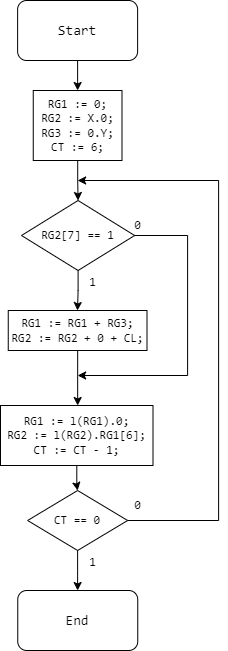
\includegraphics[width=\linewidth]{structure3_alg.png}
        \end{subfigure}
        \hfill
        \begin{subfigure}[t]{0.45\textwidth}
            \centering
            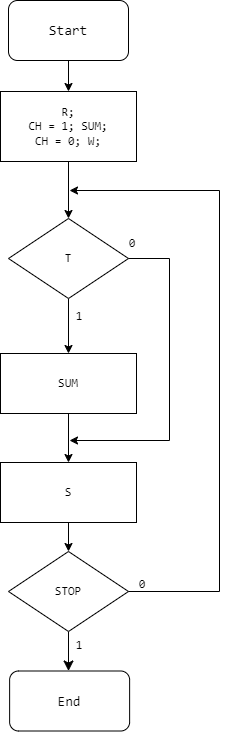
\includegraphics[width=\linewidth]{FS3_alg.png}
        \end{subfigure}
    
        \label{fig:microalg2}

    \end{figure}

    \newpage

    TABLE 2

    \newpage

    Функціональна схема множення, в якій використовується 8-бітний регістр, суматор та мультиплексор для зручності, та в подальшому мастштабуванні:

    \begin{figure}[ht]
        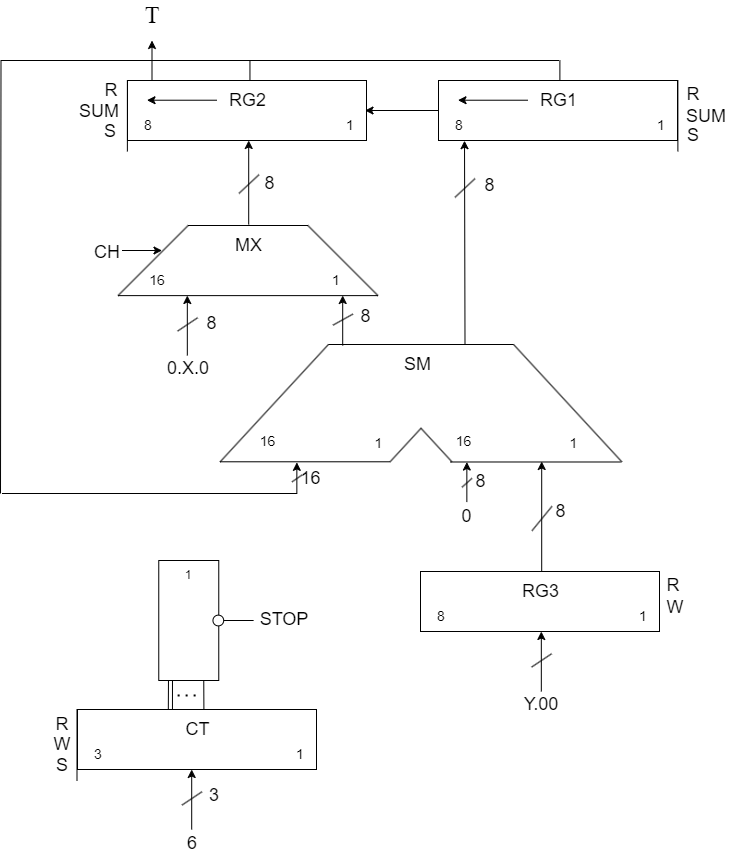
\includegraphics[width=0.9\textwidth]{multiply3_function_schemma.png}
    \end{figure}

    \newpage

    AFDK:

    \begin{figure}[ht]
        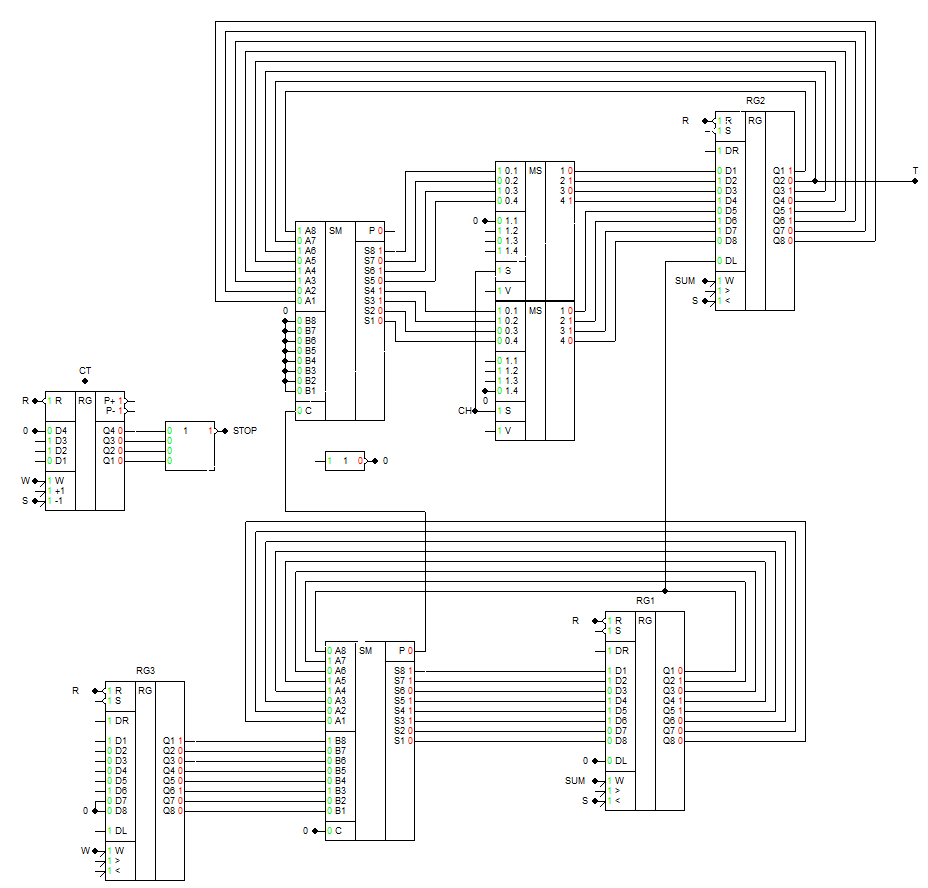
\includegraphics[width=0.9\textwidth]{schemma2.png}
    \end{figure}

    Часова діаграма:

    \begin{figure}[ht]
        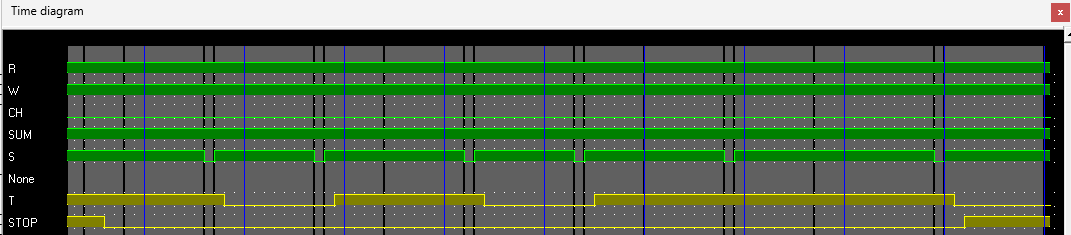
\includegraphics[width=0.9\textwidth]{time2.png}
    \end{figure}

    Результат множення збігається з попередньо обчисленим.

    \newpage

    \textbf{\Large Ділення:}

    \vspace{1em}

    \text{\large Теоретичне підґрунтя:}

    \setlength{\parindent}{1.5em}

    \vspace{1em}

    Дано два числа: $X = 2^a M_X$ та $Y = 2^b M_Y$.

    Під час ділення двох чисел отримаємо: $X \slash Y = 2^a M_X \slash 2^b M_Y = 2^{a - b} \left( M_X \slash M_Y \right)$.

    Тобто при діленні двох чисел у форматі з плаваючою комою: віднімаються порядки, діляться мантиси цих чисел.
    Ділення можна виконати, за умови $M_X < M_Y$.
    Якщо така умова не є істинною від початку, тоді зсовуємо мантису $M_X$ вправо, та додаємо 1 до значення порядку числа $X$.

    \vspace{1em}
    \setlength{\parindent}{0pt}

    \textbf{\large Ділення 1-й спосіб:}

    \vspace{1em}

    Операційна схема множення 3-го способу для 6 розрядних чисел:

    \begin{figure}[ht]
        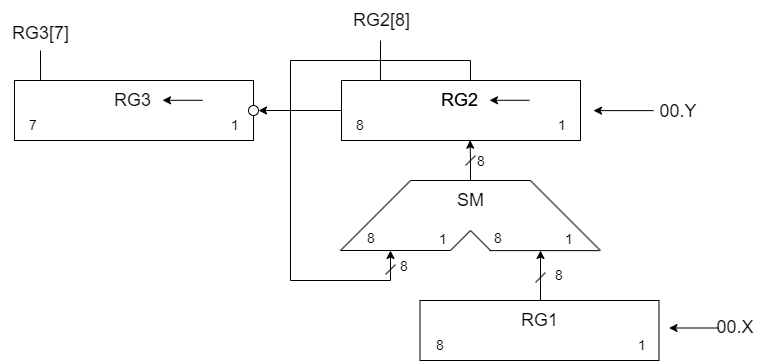
\includegraphics[width=1.0\textwidth]{division1_operation_schemma.png}
    \end{figure}

    \newpage

    Змістовний та ФС мікроалгоритми:

    \begin{figure}[h!]
        \centering
        
        \begin{subfigure}[t]{0.5\textwidth}
            \centering
            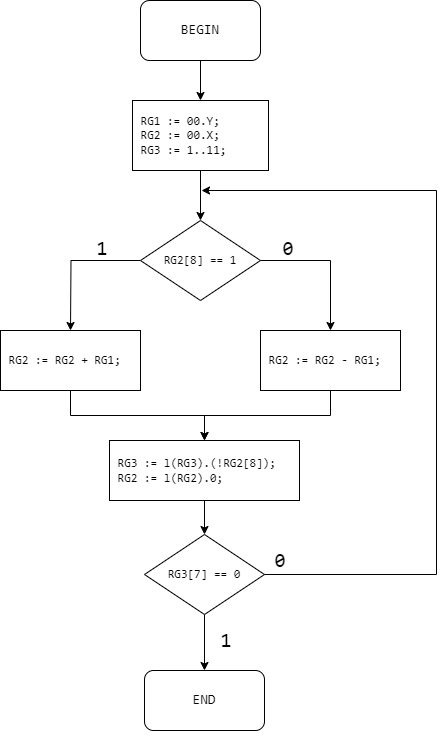
\includegraphics[width=\linewidth]{structure_div_alg.png}
        \end{subfigure}
        \hfill
        \begin{subfigure}[t]{0.45\textwidth}
            \centering
            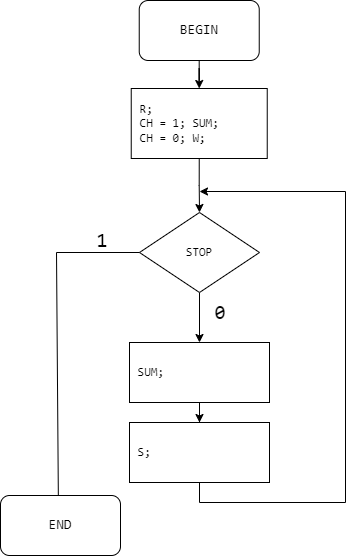
\includegraphics[width=\linewidth]{FS_div_alg.png}
        \end{subfigure}
    
        \label{fig:microalg3}

    \end{figure}

    \newpage

    TABLE 3

    \newpage

    Функціональна схема ділення:

    \begin{figure}[ht]
        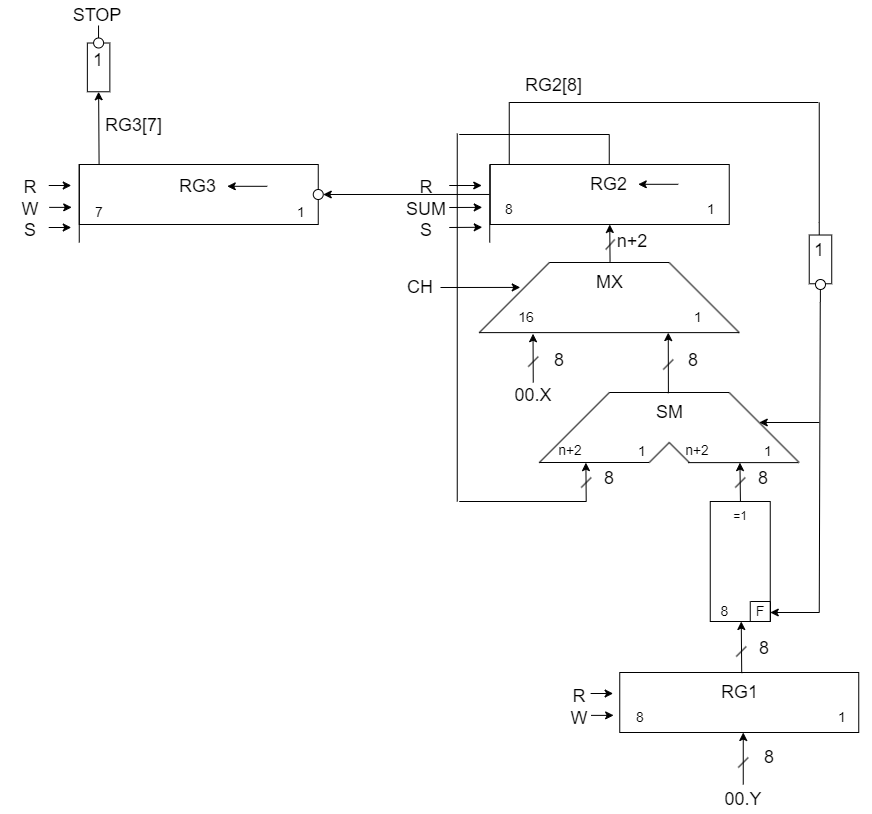
\includegraphics[width=0.9\textwidth]{division_function_schemma.png}
    \end{figure}

    \newpage

    AFDK:

    \begin{figure}[ht]
        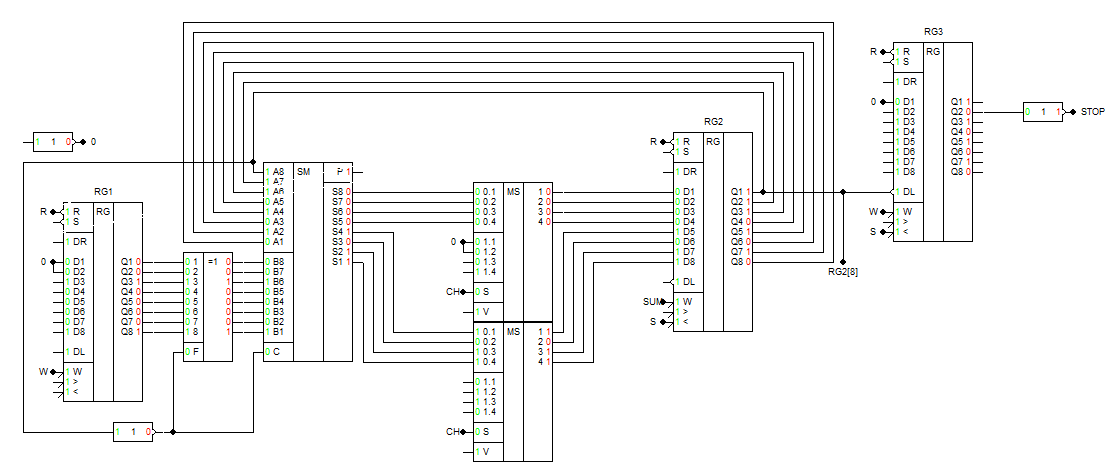
\includegraphics[width=1.0\textwidth]{schemma3.png}
    \end{figure}

    Часова діаграма:

    \begin{figure}[ht]
        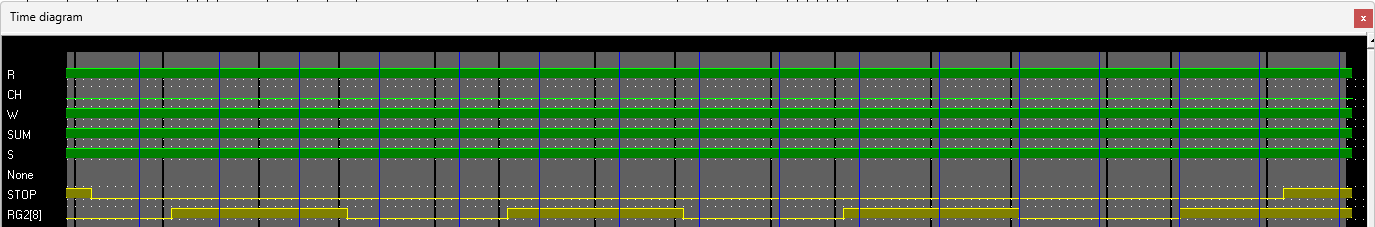
\includegraphics[width=1.0\textwidth]{time3.png}
    \end{figure}

    Результат ділення збігається з попередньо обчисленим.

    \newpage

    \textbf{\Large Додавання:}

    \vspace{1em}

    \text{\large Теоретичне підґрунтя:}

    \setlength{\parindent}{1.5em}

    \vspace{1em}

    Дано два числа: $X = 2^a M_X$ та $Y = 2^b M_Y$.

    Під час додавання двох чисел отримаємо: $X + Y = 2^a M_X + 2^b M_Y$.

    Щоб провести додавання мантис, потрібно домогтись того, щоб порядки були однакові.
    Зазвичай обирають опорним порядком є більший порядок.
    Щоб звести менший порядок до більшого, потрібно знайти їх різницю в десятковому представленні.
    І настільки ж зсунути мантису меншого порядку вправо.
    Після цього можна виконувати додання/віднімання.
    Як результівний порядок приймаємо найбільший.

    \vspace{1em}
    \setlength{\parindent}{0pt}

    \textbf{\large Додавання ДК:}

    \vspace{1em}
    \setlength{\parindent}{1.5em}

    У нас є два нормалізованих числа у форматі з плаваючою комою:
    \begin{flalign*}
        &
        \begin{array}{r@{\ =\ }c c c c}
        F & \fbox{0}     & \fbox{1010} & \fbox{1} & \fbox{101011} \\
        Y & \fbox{0}     & \fbox{0011} & \fbox{0} & \fbox{100001}
        \end{array}
        &
    \end{flalign*}

    Звідси $P_F > P_Y$, тоді визнаємо порядок $P_F$ опорним. Кількість зсувів: $P_F - P_Y = 10_{10} - 3_{10} = 7_{10}$. Тобто мантису числа $Y$ потрібно зсунути вправо на 7 бітів:

    \begin{table}[h]         % необовʼязково, лише щоб легко рухати таблицю
        \centering               % центрує всю таблицю
        \begin{tabular}{|c|c|}
        \hline
        \textbf{№ зсуву} & \textbf{Результат зсуву $M_Y$} \\ \hline
        -- & 100001 \\ \hline
        1  & 010000 \\ \hline
        2  & 001000 \\ \hline
        3  & 000100 \\ \hline
        4  & 000010 \\ \hline
        5  & 000001 \\ \hline
        6  & 000000 \\ \hline
        7  & 000000 \\ \hline
        \end{tabular}
    \end{table}

    Значить додавання мантис в ДК буде (задля спрощення запису, приймемо, що $R_{\text{ДК}}, F_{\text{ДК}}$ та $Y_{\text{ДК}}$ --- це мантиси відповідних чисел у відповідних формах):

    $R_{\text{ДК}} = F_{\text{ДК}} + Y_{\text{ДК}}$. Визначемо кожен доданок:

    \setlength{\parindent}{1.5em}

    \vspace{1em}

    $F_{\text{ДК}}:$
    \begin{flalign*}
        &
        \begin{array}{r}
        1,010100 \\
        + \phantom{1\ }0,000001 \\
        \hline
        1,010101
        \end{array}
        &
    \end{flalign*}

    $F_{\text{ДК}} = 1,010101$

    $Y_{\text{ДК}} = Y_{\text{ПК}} = 0,000000$

    Тут варто зазначити щодо нормалізації. Мантиса $F_{\text{ДК}}$ вважається нормалізованою через те, що у старшому розряді стоїть 0, за умови, що від'ємне число подане в ДК.
    Щодо мантиси $Y_{\text{ДК}}$, то вона хоч і не є нормалізованою, але домогтись нормалізації неможливо, через те, що всі її розряди дорівнюють 0 і операцію зсуву можна виконувати
    нескінченно --- через це вважатимемо її \textit{машинним нулем}.

    \vspace{1em}
    
    Тому дані числа у форматі плаваючої комі в ДК вважаються нормалізованими:
    \begin{flalign*}
        &
        \begin{array}{r@{\ =\ }c c c c}
        F_{\text{ДК}} & \fbox{0}     & \fbox{1010} & \fbox{1} & \fbox{010101} \\
        Y_{\text{ДК}} & \fbox{0}     & \fbox{1010} & \fbox{0} & \fbox{000000}
        \end{array}
        &
    \end{flalign*}

    Тепер можна виконувати додавання мантис.
    Використовуватиму модифіковані коди, які забезпечуть збереження знаку:

    $F_{\text{мод.ДК}} = 11,010101$, $Y_{\text{мод.ДК}} = 00,000000$

    \vspace{1em}

    Тоді $R_{\text{мод.ДК}}$:
    \begin{flalign*}
        &
        \begin{array}{r}
        11,010101 \\
        + \phantom{1\ }00,000000 \\
        \hline
        11,010101
        \end{array}
        &
    \end{flalign*}

    Тобто $R_{\text{мод.ДК}} = 11,010101$.

    \vspace{1em}

    Щоб перевести число ДК назад в ПК, всі розряди, окрім знакових, інвертуються та до результату інвертування додається одиниця, якщо знаковий біт дорівнює 1.
    Якщо знаковий біт = 0, то число в ДК співпадає з числом в ПК. Так як у нас знаковий біт = 1, то:

    Тоді $R_{\text{мод.ПК}}$:
    \begin{flalign*}
        &
        \begin{array}{r}
        11,101010 \\
        + \phantom{1\ }00,000001 \\
        \hline
        11,101011
        \end{array}
        &
    \end{flalign*}

    Звідси $R_{\text{ПК}} = M_R = 1,101011$, а також $P_R = P_F = 1010$. Тоді число $R$ у форматі з плаваючою комою:
    \begin{flalign*}
        &
        \begin{array}{r@{\ =\ }c c c c}
        R & \fbox{0}     & \fbox{1010} & \fbox{1} & \fbox{101011}
        \end{array}
        &
    \end{flalign*}

    Що співпадає з числом $F$. Пояснення тому через те, що для представлення мантиси виділяється лише 7 бітів, один з яких є знаковим.
    Дана кількість бітів виявилась недостанньо точною для представлення суми двох чисел, порядки яких відрізняються на 7 бітів, що є дуже великим розривом.
    Тому під час сумування сформувалась природня похибка, тому радше буде записати не =, а $\approx$.

    \newpage

    AFDK:

    \begin{figure}[ht]
        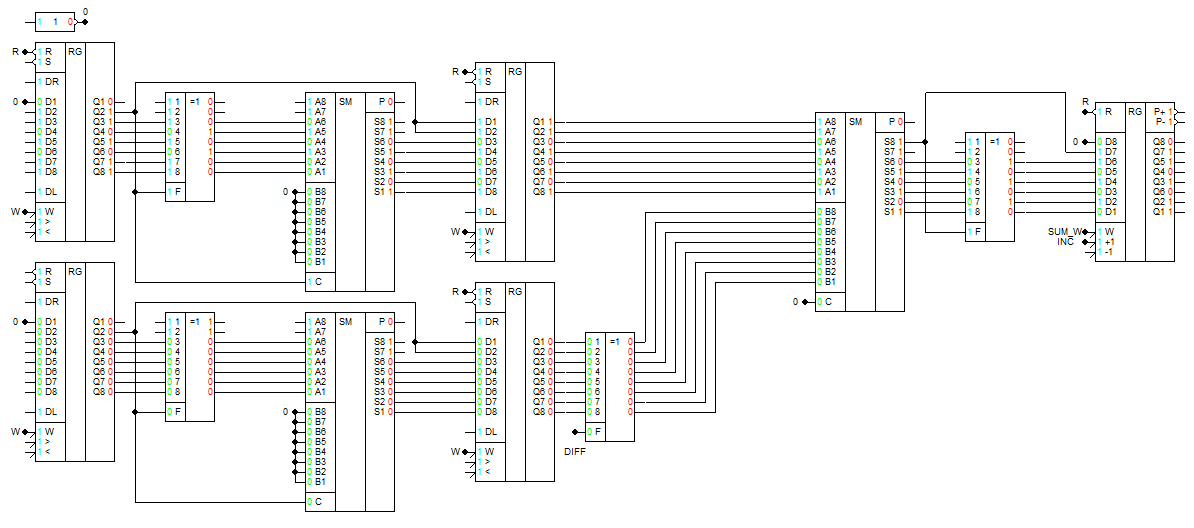
\includegraphics[width=1.0\textwidth]{schemma4.png}
    \end{figure}

    Часова діаграма:

    \begin{figure}[ht]
        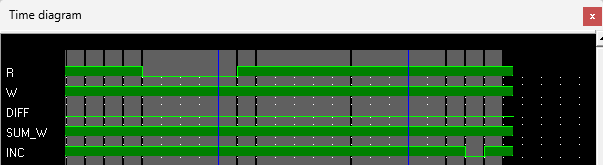
\includegraphics[width=1.0\textwidth]{time4.png}
    \end{figure}

    Результат додавання збігається з попередньо обчисленим.

    \vspace{4em}
    \setlength{\parindent}{0pt}

    \textbf{\underline{Висновок:}}
    Під час виконання цієї лабораторної роботи я поглибив та закріпив знання, отримані під час попередніх лабораторних занять. Зокрема, я повторив порядок виконання основних математичних операцій, а також набув практичних навичок роботи з числами з плаваючою комою. Окрім цього, я краще зрозумів особливості обробки таких чисел у контексті обчислень та можливі труднощі, що виникають під час їх використання.

    \newpage

    \begin{center} \textbf{\large Контрольні питання} \end{center}

    \begin{enumerate}
        \item \textit{Як перейти від функціонального (змістовного) мікроалгоритму до структурного мікроалгоритму?}
        
        Треба в блоках алгоритму замінити функції на оператори(сигнали), які призводять до їх виконання.
        \vspace{1em}

        \item \textit{Поясніть правила додавання та віднімання чисел в ОК і ДК.}
        
        Числа в ОК додаються як звичайні числа у двійковій системі, правильний знак суми формується автоматично з урахуванням перенесення. Також, якщо присутнє переповнення, то воно циклічно переноситься в наймолодший розряд.
        У ДК все так само, тільки при переповенні відстутній циклічний переніс. Віднімання просто замінюється заміною числа на протилежне (інвертування всіх розрядів окрім знакових)
        \vspace{1em}

        \item \textit{3. Поясніть правила зсуву кодів в ОК і ДК.}
        
        Якщо зсув логічний, то він для всіх кодів однаковий і відбувається зі зсувом розрядів та втратою розрядів, що вийшли за межі сітки. Пусті місця заповнюються нулями.

        Якщо зсув арифметичний, то для кожного коду свої правила.
        
        Для ПК: cхожий на логічний зсув, окрім того, що знакові розряди не зсовуються.

        Для ОК: зсув праворуч --- молодший біт втрачається, старший розряд стає таким самим, як і знаковий, зсув ліворуч --- всі розряди, включно із знаковими зсовуються: найстарший знаковий розряд поміщається у кінець (наймолодший) розряд.

        Для ДК: зсув праворуч --- такий самий, як і для ОК, зсув ліворуч --- такий самий як для ОК, окрім того, що відсутній циклічний переніс старшого знакового розряду в молодший. Молодший натомість заповнюється нулем.

        \vspace{1em}

        \item \textit{Як можна виявити переповнення розрядної сітки при виконанні операцій з машинними кодами?}
        
        Для виявлення переповнення в комп'ютерних системах часто використовують модифіковані машинні коди, в яких додатковий знаковий розряд ЗР2 знаходиться ліворуч від основного розряду ЗР1.
        Якщо відбувається переповнення розрядної сітки, то старший знаковий розряд завжди зберігає знак результату, а сам факт переповення фіксується відмінністю знакових розрядів ЗР1 та ЗР2.

        \vspace{1em}

        \item \textit{Яким чином можна подати мікрооперації і мікроалгоритми?}
        
        Мікрооперації --- це найменші операції, які виконує процесор комп'ютера, щоб обробити інформацію.
        Мікрооперації можуть бути записані в таблицю і містити ім'я операції, адресний регістр, регістр даних, зсув та коментар.
        Мікроалгоритми – це послідовності мікрооперацій, які виконуються в певному порядку, при певних умовах процесором для виконання команд або функцій.
        Мікроалгоритми можуть бути представлені у вигляді блок-схем або тексту, а також можуть бути записані у вигляді таблиці.
        У таблицях використовують позначення станів, щоб вказати, які мікрооперації будуть виконані залежно від стану процесора та операндів.

        \vspace{1em}
    
        \item \textit{Форми подання чисел в ЕОМ.}
        
        З фіксованою або плаваючою комою.
        \vspace{1em}

        \item \textit{Виконання операцій з числами в форматі з фіксованою комою.}
        
        Числа із фіксованою комою подаються лише мантисою, без порядку. Це означає, що операції над числами в форматі з фіксованою комою виконуються так само, як і над їх мантисами.

        \vspace{1em}

        \item \textit{Етапи додавання чисел з плаваючою комою.}
        
        Зрівняння порядків, додавання мантис, нормалізація результату, округлення (за потреби), формування результату.

        \vspace{1em}

        \item \textit{Дайте означення мікрооперації та мікроалгоритму?}
        
        Мікрооперація --- програма на спеціалізованій, апаратно-залежній мові програмування, що реалізує керування процесором в системах з мікропрограмним керуванням.

        Мікроалгоритм --- послідовність мікрооперацій, що приводить до виконання операцій в залежності від зовнішніх аргументів та внутрішніх станів, називають мікроалгоритмом.

        \item \textit{Схарактеризувати основні етапи проєктування пристрою для виконання операції.}
        
        \begin{enumerate}
            \item Вивчити математичну основу та доведення певної операції над числом.
            \item Побудувати операційну схему для певної операції.
            \item Розробити змістовний мікроалгоритм.
            \item Розробити функціонально-структурний мікроалгоритм, замінюючи мікрооперації сигналами.
            \item Побудувати функціональну схему.
            \item Побудувати логічну схему в засобах побудови логічних пристроїв.
        \end{enumerate}

        \vspace{1em}

        \item \textit{Як визначити необхідну тривалість керуючих сигналів?}
        
        Керуючий сигнал повинен бути достатньо довгим для того, щоб встиг прийти сигнал зворотного зв'язку.

        \vspace{1em}

        \item \textit{Як перейти від операційної схеми до функціональної?}
        
        На основі операційної схема та ФС мікроалгоритму та на основі базису доступних операційних пристроїв (регістр, суматор і т.д.) побудувати схему, яка детально відображає особливості та структуру
        логічної, реальної схеми.

        \vspace{1em}

        \item \textit{Як розрахувати розрядність вузлів операційного пристрою?}
        
        Все залежить від різних способів виконання операцій --- це зумовлюється різними чинниками, такі як особливість методу, збільшення точності, запобіганню переповнення, тощо.

    \end{enumerate}

\end{document}